% Options for packages loaded elsewhere
\PassOptionsToPackage{unicode}{hyperref}
\PassOptionsToPackage{hyphens}{url}
%
\documentclass[
]{article}
\usepackage{lmodern}
\usepackage{amssymb,amsmath}
\usepackage{ifxetex,ifluatex}
\ifnum 0\ifxetex 1\fi\ifluatex 1\fi=0 % if pdftex
  \usepackage[T1]{fontenc}
  \usepackage[utf8]{inputenc}
  \usepackage{textcomp} % provide euro and other symbols
\else % if luatex or xetex
  \usepackage{unicode-math}
  \defaultfontfeatures{Scale=MatchLowercase}
  \defaultfontfeatures[\rmfamily]{Ligatures=TeX,Scale=1}
\fi
% Use upquote if available, for straight quotes in verbatim environments
\IfFileExists{upquote.sty}{\usepackage{upquote}}{}
\IfFileExists{microtype.sty}{% use microtype if available
  \usepackage[]{microtype}
  \UseMicrotypeSet[protrusion]{basicmath} % disable protrusion for tt fonts
}{}
\makeatletter
\@ifundefined{KOMAClassName}{% if non-KOMA class
  \IfFileExists{parskip.sty}{%
    \usepackage{parskip}
  }{% else
    \setlength{\parindent}{0pt}
    \setlength{\parskip}{6pt plus 2pt minus 1pt}}
}{% if KOMA class
  \KOMAoptions{parskip=half}}
\makeatother
\usepackage{xcolor}
\IfFileExists{xurl.sty}{\usepackage{xurl}}{} % add URL line breaks if available
\IfFileExists{bookmark.sty}{\usepackage{bookmark}}{\usepackage{hyperref}}
\hypersetup{
  pdftitle={Practical 01 SG: Descriptive analysis of genetic markers},
  pdfauthor={Ivan Almer, Lovro Katalinić},
  hidelinks,
  pdfcreator={LaTeX via pandoc}}
\urlstyle{same} % disable monospaced font for URLs
\usepackage[margin=1in]{geometry}
\usepackage{color}
\usepackage{fancyvrb}
\newcommand{\VerbBar}{|}
\newcommand{\VERB}{\Verb[commandchars=\\\{\}]}
\DefineVerbatimEnvironment{Highlighting}{Verbatim}{commandchars=\\\{\}}
% Add ',fontsize=\small' for more characters per line
\usepackage{framed}
\definecolor{shadecolor}{RGB}{248,248,248}
\newenvironment{Shaded}{\begin{snugshade}}{\end{snugshade}}
\newcommand{\AlertTok}[1]{\textcolor[rgb]{0.94,0.16,0.16}{#1}}
\newcommand{\AnnotationTok}[1]{\textcolor[rgb]{0.56,0.35,0.01}{\textbf{\textit{#1}}}}
\newcommand{\AttributeTok}[1]{\textcolor[rgb]{0.77,0.63,0.00}{#1}}
\newcommand{\BaseNTok}[1]{\textcolor[rgb]{0.00,0.00,0.81}{#1}}
\newcommand{\BuiltInTok}[1]{#1}
\newcommand{\CharTok}[1]{\textcolor[rgb]{0.31,0.60,0.02}{#1}}
\newcommand{\CommentTok}[1]{\textcolor[rgb]{0.56,0.35,0.01}{\textit{#1}}}
\newcommand{\CommentVarTok}[1]{\textcolor[rgb]{0.56,0.35,0.01}{\textbf{\textit{#1}}}}
\newcommand{\ConstantTok}[1]{\textcolor[rgb]{0.00,0.00,0.00}{#1}}
\newcommand{\ControlFlowTok}[1]{\textcolor[rgb]{0.13,0.29,0.53}{\textbf{#1}}}
\newcommand{\DataTypeTok}[1]{\textcolor[rgb]{0.13,0.29,0.53}{#1}}
\newcommand{\DecValTok}[1]{\textcolor[rgb]{0.00,0.00,0.81}{#1}}
\newcommand{\DocumentationTok}[1]{\textcolor[rgb]{0.56,0.35,0.01}{\textbf{\textit{#1}}}}
\newcommand{\ErrorTok}[1]{\textcolor[rgb]{0.64,0.00,0.00}{\textbf{#1}}}
\newcommand{\ExtensionTok}[1]{#1}
\newcommand{\FloatTok}[1]{\textcolor[rgb]{0.00,0.00,0.81}{#1}}
\newcommand{\FunctionTok}[1]{\textcolor[rgb]{0.00,0.00,0.00}{#1}}
\newcommand{\ImportTok}[1]{#1}
\newcommand{\InformationTok}[1]{\textcolor[rgb]{0.56,0.35,0.01}{\textbf{\textit{#1}}}}
\newcommand{\KeywordTok}[1]{\textcolor[rgb]{0.13,0.29,0.53}{\textbf{#1}}}
\newcommand{\NormalTok}[1]{#1}
\newcommand{\OperatorTok}[1]{\textcolor[rgb]{0.81,0.36,0.00}{\textbf{#1}}}
\newcommand{\OtherTok}[1]{\textcolor[rgb]{0.56,0.35,0.01}{#1}}
\newcommand{\PreprocessorTok}[1]{\textcolor[rgb]{0.56,0.35,0.01}{\textit{#1}}}
\newcommand{\RegionMarkerTok}[1]{#1}
\newcommand{\SpecialCharTok}[1]{\textcolor[rgb]{0.00,0.00,0.00}{#1}}
\newcommand{\SpecialStringTok}[1]{\textcolor[rgb]{0.31,0.60,0.02}{#1}}
\newcommand{\StringTok}[1]{\textcolor[rgb]{0.31,0.60,0.02}{#1}}
\newcommand{\VariableTok}[1]{\textcolor[rgb]{0.00,0.00,0.00}{#1}}
\newcommand{\VerbatimStringTok}[1]{\textcolor[rgb]{0.31,0.60,0.02}{#1}}
\newcommand{\WarningTok}[1]{\textcolor[rgb]{0.56,0.35,0.01}{\textbf{\textit{#1}}}}
\usepackage{graphicx,grffile}
\makeatletter
\def\maxwidth{\ifdim\Gin@nat@width>\linewidth\linewidth\else\Gin@nat@width\fi}
\def\maxheight{\ifdim\Gin@nat@height>\textheight\textheight\else\Gin@nat@height\fi}
\makeatother
% Scale images if necessary, so that they will not overflow the page
% margins by default, and it is still possible to overwrite the defaults
% using explicit options in \includegraphics[width, height, ...]{}
\setkeys{Gin}{width=\maxwidth,height=\maxheight,keepaspectratio}
% Set default figure placement to htbp
\makeatletter
\def\fps@figure{htbp}
\makeatother
\setlength{\emergencystretch}{3em} % prevent overfull lines
\providecommand{\tightlist}{%
  \setlength{\itemsep}{0pt}\setlength{\parskip}{0pt}}
\setcounter{secnumdepth}{-\maxdimen} % remove section numbering

\title{Practical 01 SG: Descriptive analysis of genetic markers}
\author{Ivan Almer, Lovro Katalinić}
\date{Hand-in: 20/11/2020}

\begin{document}
\maketitle

Resolve the following exercise in groups of two students. Perform the
computations and make the graphics that are asked for in the practical
below. Take care to give each graph a title, and clearly label \(x\) and
\(y\) axes, and to answer all questions asked. You can write your
solution in a Word or Latex document and generate a pdf file with your
solution, or generate a solution pdf file with R Markdown. Take care to
number your answers exactly as in this exercise. Upload your solution in
\textbf{pdf format} to the web page of the course at raco.fib.upc.edu no
later than the hand-in date.

You can make use of the R-package \textbf{genetics} (and other packages)
to compute your answers, as you please. The first part of the practical
is dedicated to the descriptive analysis of SNP data, whereas the second
part is dedicated to the analysis of STR data. The datasets can be
downloaded by clicking on their file names given below.

\hypertarget{snp-dataset-10p}{%
\section{SNP dataset (10p)}\label{snp-dataset-10p}}

\begin{enumerate}
\def\labelenumi{\arabic{enumi}.}
\item
  The file
  \href{http://www-eio.upc.es/~jan/data/bsg/CHDCHR22RAW.raw}{CHDCHR22RAW.raw}
  contains all SNPs on chromosome 22 of a sample of Chinese individuals
  in Metropolitan Denver, CO, USA. This data has been extracted from the
  1000 genomes project at
  \href{http://www.internationalgenome.org}{www.internationalgenome.org}
  .
\item
  Load this data into the R environment, with the \texttt{read.table}
  instruction. The first six columns contain non-genetical information.
  Extract the variables individual ID (the second column IID) and the
  sex of the individual (the 5th column sex). Create a dataframe that
  only contains the genetic information that is in and beyond the 7th
  column. Notice that the genetic variants are identifed by an ``rs''
  identifier. The genetic data is coded in the (0, 1, 2) format with
  0=AA, 1=AB, 2=BB.
\item
  (1p) How many variants are there in this database? What percentage of
  the data is missing? How many individuals in the database are males
  and how many are females?
\end{enumerate}

\begin{Shaded}
\begin{Highlighting}[]
\NormalTok{dataset =}\StringTok{ }\KeywordTok{read.table}\NormalTok{(}\StringTok{"CHDCHR22.raw"}\NormalTok{)}

\NormalTok{ids =}\StringTok{ }\NormalTok{dataset[,}\DecValTok{2}\NormalTok{]}
\NormalTok{ids =}\StringTok{ }\NormalTok{ids[}\DecValTok{2}\OperatorTok{:}\KeywordTok{length}\NormalTok{(ids)]}
\NormalTok{sexes =}\StringTok{ }\NormalTok{dataset[,}\DecValTok{5}\NormalTok{]}
\NormalTok{sexes =}\StringTok{ }\NormalTok{sexes[}\DecValTok{2}\OperatorTok{:}\KeywordTok{length}\NormalTok{(sexes)]}

\NormalTok{genetic_dataset =}\StringTok{ }\KeywordTok{data.frame}\NormalTok{(dataset[,}\DecValTok{7}\OperatorTok{:}\KeywordTok{ncol}\NormalTok{(dataset)])}
\NormalTok{names =}\StringTok{ }\NormalTok{genetic_dataset[}\DecValTok{1}\NormalTok{,]}
\NormalTok{genetic_dataset =}\StringTok{ }\KeywordTok{data.frame}\NormalTok{(genetic_dataset[}\DecValTok{2}\OperatorTok{:}\KeywordTok{nrow}\NormalTok{(genetic_dataset),])}
\KeywordTok{names}\NormalTok{(genetic_dataset) =}\StringTok{ }\NormalTok{names}

\CommentTok{# Number of variants}
\NormalTok{num_var =}\StringTok{ }\KeywordTok{ncol}\NormalTok{(genetic_dataset)}
\KeywordTok{cat}\NormalTok{(}\KeywordTok{paste}\NormalTok{(}\StringTok{'Number of variants:'}\NormalTok{, num_var, }\StringTok{'}\CharTok{\textbackslash{}n}\StringTok{'}\NormalTok{))}
\end{Highlighting}
\end{Shaded}

\begin{verbatim}
## Number of variants: 16393
\end{verbatim}

\begin{Shaded}
\begin{Highlighting}[]
\CommentTok{# Percentage of data missing}
\NormalTok{genetic_dataset[genetic_dataset }\OperatorTok{==}\StringTok{ }\DecValTok{-9}\NormalTok{] <-}\StringTok{ }\OtherTok{NA}
\NormalTok{nmis =}\StringTok{ }\KeywordTok{sum}\NormalTok{(}\KeywordTok{is.na}\NormalTok{(genetic_dataset))}
\NormalTok{percentage_missing =}\StringTok{ }\NormalTok{nmis }\OperatorTok{/}\StringTok{ }\NormalTok{(}\KeywordTok{nrow}\NormalTok{(genetic_dataset) }\OperatorTok{*}\StringTok{ }\KeywordTok{ncol}\NormalTok{(genetic_dataset))}
\KeywordTok{cat}\NormalTok{(}\KeywordTok{paste}\NormalTok{(}\StringTok{'Percentage of data missing:'}\NormalTok{, percentage_missing, }\StringTok{'%}\CharTok{\textbackslash{}n}\StringTok{'}\NormalTok{))}
\end{Highlighting}
\end{Shaded}

\begin{verbatim}
## Percentage of data missing: 0 %
\end{verbatim}

\begin{Shaded}
\begin{Highlighting}[]
\CommentTok{# Number of ales and females}
\NormalTok{male_sign =}\StringTok{ }\DecValTok{1}
\NormalTok{female_sign =}\StringTok{ }\DecValTok{2}
\NormalTok{n_male =}\StringTok{ }\KeywordTok{sum}\NormalTok{(sexes}\OperatorTok{==}\NormalTok{male_sign)}
\NormalTok{n_female =}\StringTok{ }\KeywordTok{sum}\NormalTok{(sexes}\OperatorTok{==}\NormalTok{female_sign)}
\KeywordTok{cat}\NormalTok{(}\KeywordTok{paste}\NormalTok{(}\StringTok{'Male individuals: '}\NormalTok{, n_male, }\StringTok{'}\CharTok{\textbackslash{}n}\StringTok{Female individuals: '}\NormalTok{, n_female))}
\end{Highlighting}
\end{Shaded}

\begin{verbatim}
## Male individuals:  50 
## Female individuals:  59
\end{verbatim}

\begin{enumerate}
\def\labelenumi{\arabic{enumi}.}
\setcounter{enumi}{3}
\tightlist
\item
  (1p) Calculate the percentage of monomorphic variants. Exclude all
  monomorphics from the database for all posterior computations of the
  practical. How many variants do remain in your database?
\end{enumerate}

\begin{Shaded}
\begin{Highlighting}[]
\NormalTok{genetic_dataset_non_monomorphic =}\StringTok{ }\OtherTok{NULL}

\ControlFlowTok{for}\NormalTok{(i }\ControlFlowTok{in} \DecValTok{1}\OperatorTok{:}\KeywordTok{ncol}\NormalTok{(genetic_dataset)) \{}
\NormalTok{  is_monomorphic =}\StringTok{ }\KeywordTok{length}\NormalTok{(}\KeywordTok{unique}\NormalTok{(genetic_dataset[,i])) }\OperatorTok{==}\StringTok{ }\DecValTok{1}
  \ControlFlowTok{if}\NormalTok{ (is_monomorphic }\OperatorTok{==}\StringTok{ }\OtherTok{FALSE}\NormalTok{) \{}
\NormalTok{    col_name =}\StringTok{ }\KeywordTok{names}\NormalTok{(genetic_dataset)[i]}
    \CommentTok{# add to dataframe}
    \ControlFlowTok{if}\NormalTok{(}\KeywordTok{is.null}\NormalTok{(genetic_dataset_non_monomorphic)) \{}
\NormalTok{      genetic_dataset_non_monomorphic =}\StringTok{ }\KeywordTok{data.frame}\NormalTok{(genetic_dataset[,i])}
      \KeywordTok{names}\NormalTok{(genetic_dataset_non_monomorphic) =}\StringTok{ }\KeywordTok{c}\NormalTok{(col_name)}
\NormalTok{    \} }\ControlFlowTok{else}\NormalTok{ \{}
\NormalTok{      names_before =}\StringTok{ }\KeywordTok{names}\NormalTok{(genetic_dataset_non_monomorphic)}
\NormalTok{      genetic_dataset_non_monomorphic =}\StringTok{ }\KeywordTok{cbind}\NormalTok{(genetic_dataset_non_monomorphic, }\KeywordTok{data.frame}\NormalTok{(genetic_dataset[,i]))}
      \KeywordTok{names}\NormalTok{(genetic_dataset_non_monomorphic) =}\StringTok{ }\KeywordTok{append}\NormalTok{(names_before, col_name)}
\NormalTok{    \}}
\NormalTok{  \}}
\NormalTok{\}}


\CommentTok{# There are 13192 Variants remaining in my database}
\NormalTok{perc =}\StringTok{ }\DecValTok{1} \OperatorTok{-}\StringTok{ }\KeywordTok{ncol}\NormalTok{(genetic_dataset_non_monomorphic) }\OperatorTok{/}\StringTok{ }\KeywordTok{ncol}\NormalTok{(genetic_dataset)}
\KeywordTok{cat}\NormalTok{(}\KeywordTok{paste}\NormalTok{(}\StringTok{'Percentage of monomorphic variants: '}\NormalTok{, perc, }\StringTok{'}\CharTok{\textbackslash{}n}\StringTok{'}\NormalTok{))}
\end{Highlighting}
\end{Shaded}

\begin{verbatim}
## Percentage of monomorphic variants:  0.195266272189349
\end{verbatim}

\begin{Shaded}
\begin{Highlighting}[]
\KeywordTok{cat}\NormalTok{(}\KeywordTok{paste}\NormalTok{(}\StringTok{'Number of variants after excluding monomorphics: '}\NormalTok{, }\KeywordTok{ncol}\NormalTok{(genetic_dataset_non_monomorphic)))}
\end{Highlighting}
\end{Shaded}

\begin{verbatim}
## Number of variants after excluding monomorphics:  13192
\end{verbatim}

\begin{enumerate}
\def\labelenumi{\arabic{enumi}.}
\setcounter{enumi}{4}
\tightlist
\item
  (1p) Report the genotype counts and the minor allele count of
  polymorphism rs3729688\_G, and calculate the MAF of this variant.
\end{enumerate}

\begin{verbatim}
## Loading required package: combinat
\end{verbatim}

\begin{verbatim}
## 
## Attaching package: 'combinat'
\end{verbatim}

\begin{verbatim}
## The following object is masked from 'package:utils':
## 
##     combn
\end{verbatim}

\begin{verbatim}
## Loading required package: gdata
\end{verbatim}

\begin{verbatim}
## gdata: read.xls support for 'XLS' (Excel 97-2004) files ENABLED.
\end{verbatim}

\begin{verbatim}
## 
\end{verbatim}

\begin{verbatim}
## gdata: read.xls support for 'XLSX' (Excel 2007+) files ENABLED.
\end{verbatim}

\begin{verbatim}
## 
## Attaching package: 'gdata'
\end{verbatim}

\begin{verbatim}
## The following object is masked from 'package:stats':
## 
##     nobs
\end{verbatim}

\begin{verbatim}
## The following object is masked from 'package:utils':
## 
##     object.size
\end{verbatim}

\begin{verbatim}
## The following object is masked from 'package:base':
## 
##     startsWith
\end{verbatim}

\begin{verbatim}
## Loading required package: gtools
\end{verbatim}

\begin{verbatim}
## Loading required package: MASS
\end{verbatim}

\begin{verbatim}
## Loading required package: mvtnorm
\end{verbatim}

\begin{verbatim}
## 
\end{verbatim}

\begin{verbatim}
## NOTE: THIS PACKAGE IS NOW OBSOLETE.
\end{verbatim}

\begin{verbatim}
## 
\end{verbatim}

\begin{verbatim}
##   The R-Genetics project has developed an set of enhanced genetics
\end{verbatim}

\begin{verbatim}
##   packages to replace 'genetics'. Please visit the project homepage
\end{verbatim}

\begin{verbatim}
##   at http://rgenetics.org for informtion.
\end{verbatim}

\begin{verbatim}
## 
\end{verbatim}

\begin{verbatim}
## 
## Attaching package: 'genetics'
\end{verbatim}

\begin{verbatim}
## The following objects are masked from 'package:base':
## 
##     %in%, as.factor, order
\end{verbatim}

\begin{verbatim}
## 
## Number of samples typed: 109 (100%)
## 
## Allele Frequency: (2 alleles)
##   Count Proportion
## A   119       0.55
## B    99       0.45
## 
## 
## Genotype Frequency:
##     Count Proportion
## A/A    29       0.27
## A/B    61       0.56
## B/B    19       0.17
## 
## Heterozygosity (Hu)  = 0.4980764
## Poly. Inf. Content   = 0.3728869
\end{verbatim}

\begin{verbatim}
## 
## MAF of variant: 0.454128440366972
\end{verbatim}

\begin{enumerate}
\def\labelenumi{\arabic{enumi}.}
\setcounter{enumi}{5}
\tightlist
\item
  (2p) Compute the minor allele frequencies (MAF) for all markers, and
  make a histogram of it. Does the MAF follow a uniform distribution?
  What percentage of the markers have a MAF below 0.05? And below 0.01?
  Can you explain the observed pattern?
\end{enumerate}

\begin{Shaded}
\begin{Highlighting}[]
\NormalTok{maf.per.snp <-}\StringTok{ }\KeywordTok{apply}\NormalTok{(genetic_dataset_non_monomorphic,}\DecValTok{2}\NormalTok{,maf)}
\KeywordTok{hist}\NormalTok{(maf.per.snp, }\DataTypeTok{main=}\StringTok{"Histogram of MAF for all markers"}\NormalTok{, }\DataTypeTok{xlab=}\StringTok{"MAF"}\NormalTok{, }\DataTypeTok{ylab=}\StringTok{"Count"}\NormalTok{)}
\end{Highlighting}
\end{Shaded}

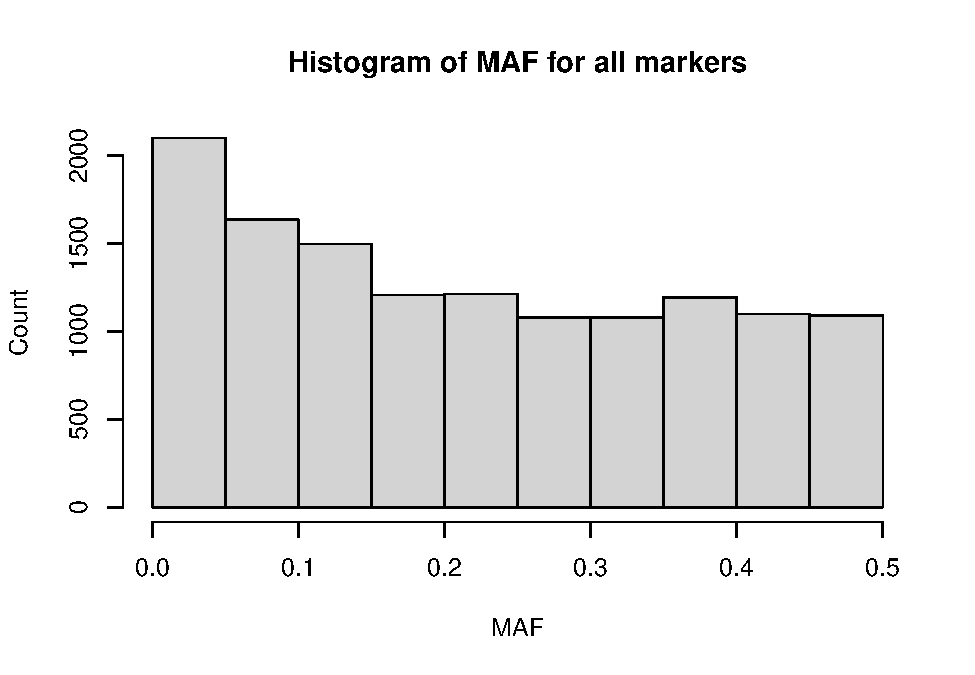
\includegraphics{P012020_Introduction_files/figure-latex/6th-1.pdf}

\begin{Shaded}
\begin{Highlighting}[]
\KeywordTok{cat}\NormalTok{(}\KeywordTok{paste}\NormalTok{(}\StringTok{'Percentage of markers with MAF below the 0.05: '}\NormalTok{, }\KeywordTok{sum}\NormalTok{(maf.per.snp }\OperatorTok{<}\StringTok{ }\FloatTok{0.05}\NormalTok{) }\OperatorTok{/}\StringTok{ }\KeywordTok{length}\NormalTok{(maf.per.snp), }\StringTok{'}\CharTok{\textbackslash{}n}\StringTok{'}\NormalTok{))}
\end{Highlighting}
\end{Shaded}

\begin{verbatim}
## Percentage of markers with MAF below the 0.05:  0.159263189812007
\end{verbatim}

\begin{Shaded}
\begin{Highlighting}[]
\KeywordTok{cat}\NormalTok{(}\KeywordTok{paste}\NormalTok{(}\StringTok{'Percentage of markers with MAF below the 0.01: '}\NormalTok{, }\KeywordTok{sum}\NormalTok{(maf.per.snp }\OperatorTok{<}\StringTok{ }\FloatTok{0.01}\NormalTok{) }\OperatorTok{/}\StringTok{ }\KeywordTok{length}\NormalTok{(maf.per.snp), }\StringTok{'}\CharTok{\textbackslash{}n}\StringTok{'}\NormalTok{))}
\end{Highlighting}
\end{Shaded}

\begin{verbatim}
## Percentage of markers with MAF below the 0.01:  0.0596573681018799
\end{verbatim}

The MAF more or less follows uniform distribution, at least visually. It
is not perfect since there is substantial number of variants with MAF
below 0.1. There is 15.9\% of variants with MAF below 0.05, and 6\%
variants with MAF below 0.01.What this means is that there are a lot
more variants with near-monomorphic constitution.

\begin{enumerate}
\def\labelenumi{\arabic{enumi}.}
\setcounter{enumi}{6}
\tightlist
\item
  (2p) Calculate the minor allele frequency for males and for females
  and present a scatterplot of these variables. What do you observe?
  Calculate and report their correlation coefficient.
\end{enumerate}

\begin{Shaded}
\begin{Highlighting}[]
\NormalTok{maf.male <-}\StringTok{ }\ControlFlowTok{function}\NormalTok{(x)\{}
\NormalTok{  male_mask =}\StringTok{ }\NormalTok{sexes }\OperatorTok{==}\StringTok{ }\NormalTok{male_sign}
\NormalTok{  x =}\StringTok{ }\NormalTok{x[male_mask]}
\NormalTok{  af1 =}\StringTok{ }\KeywordTok{maf}\NormalTok{(x)}
  \KeywordTok{return}\NormalTok{(af1)}
\NormalTok{\}}

\NormalTok{maf.female <-}\StringTok{ }\ControlFlowTok{function}\NormalTok{(x)\{}
\NormalTok{  female_mask =}\StringTok{ }\NormalTok{sexes }\OperatorTok{==}\StringTok{ }\NormalTok{female_sign}
\NormalTok{  x =}\StringTok{ }\NormalTok{x[female_mask]}
\NormalTok{  af1 =}\StringTok{ }\KeywordTok{maf}\NormalTok{(x)}
  \KeywordTok{return}\NormalTok{(af1)}
\NormalTok{\}}

\NormalTok{maf.per.snp.male =}\StringTok{ }\KeywordTok{apply}\NormalTok{(genetic_dataset_non_monomorphic, }\DecValTok{2}\NormalTok{, maf.male)}
\NormalTok{maf.per.snp.female =}\StringTok{ }\KeywordTok{apply}\NormalTok{(genetic_dataset_non_monomorphic, }\DecValTok{2}\NormalTok{, maf.female)}

\KeywordTok{plot}\NormalTok{(maf.per.snp.male, maf.per.snp.female, }\DataTypeTok{main=}\StringTok{"MAF of males against MAF of females (each dot represents one variant)"}\NormalTok{, }\DataTypeTok{xlab=}\StringTok{"MAF female"}\NormalTok{, }\DataTypeTok{ylab=}\StringTok{"MAF male"}\NormalTok{)}
\end{Highlighting}
\end{Shaded}

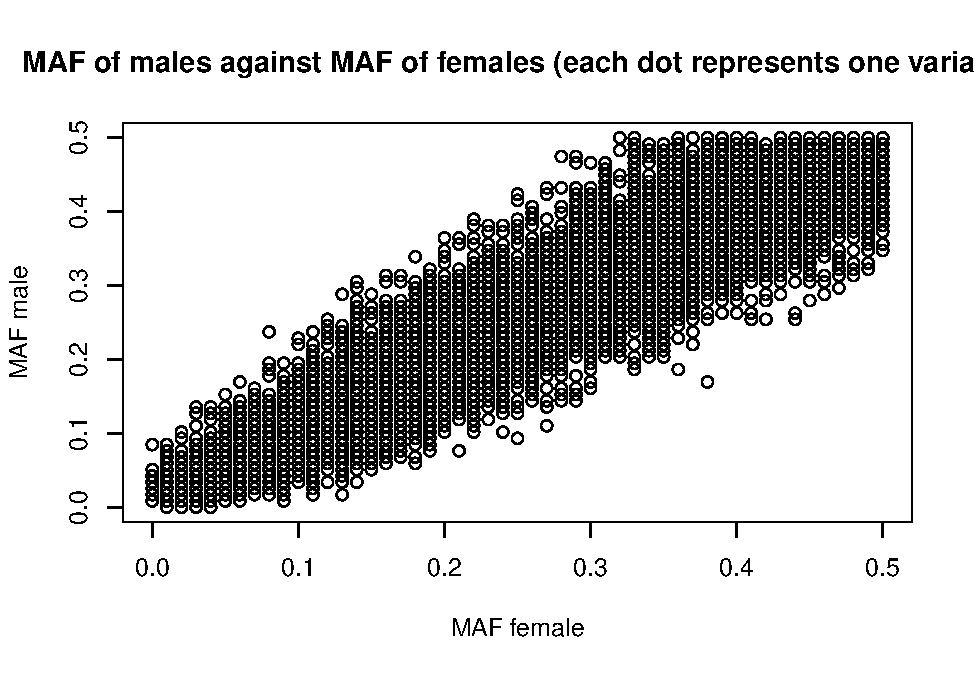
\includegraphics{P012020_Introduction_files/figure-latex/7th-1.pdf}

\begin{Shaded}
\begin{Highlighting}[]
\KeywordTok{cat}\NormalTok{(}\KeywordTok{paste}\NormalTok{(}\StringTok{'Correlation coefficient between male and female minor MAFs: '}\NormalTok{, }\KeywordTok{cor}\NormalTok{(maf.per.snp.male, maf.per.snp.female)))}
\end{Highlighting}
\end{Shaded}

\begin{verbatim}
## Correlation coefficient between male and female minor MAFs:  0.948692122941391
\end{verbatim}

We can observe that there exists some linear dependency between the
minimum allele frequency among males and females. Since visually it
makes sense that those 2 variables are correlated, we calculate the
Pearson correlation coefficient which is near 0.95. That means that
there is a high positive correlation between MAF in males and females
(i.e.~if one grows, other one also grows).

\begin{enumerate}
\def\labelenumi{\arabic{enumi}.}
\setcounter{enumi}{7}
\tightlist
\item
  (1p) Calculate the observed heterozygosity (\(H_o\)), and make a
  histogram of it. What is, theoretically, the range of variation of
  this statistic?
\end{enumerate}

\begin{Shaded}
\begin{Highlighting}[]
\NormalTok{h.observed <-}\StringTok{ }\ControlFlowTok{function}\NormalTok{(x) \{}
\NormalTok{  x[x }\OperatorTok{==}\StringTok{ }\DecValTok{0}\NormalTok{] =}\StringTok{ "AA"}
\NormalTok{  x[x }\OperatorTok{==}\StringTok{ }\DecValTok{1}\NormalTok{] =}\StringTok{ "AB"}
\NormalTok{  x[x }\OperatorTok{==}\StringTok{ }\DecValTok{2}\NormalTok{] =}\StringTok{ "BB"}
\NormalTok{  x <-}\StringTok{ }\KeywordTok{genotype}\NormalTok{(x,}\DataTypeTok{sep=}\StringTok{""}\NormalTok{)}
\NormalTok{  out <-}\StringTok{ }\KeywordTok{summary}\NormalTok{(x)}
\NormalTok{  h.o =}\StringTok{ }\NormalTok{out}\OperatorTok{$}\NormalTok{genotype.freq[,}\DecValTok{2}\NormalTok{][}\StringTok{"A/B"}\NormalTok{]}
  \ControlFlowTok{if}\NormalTok{(}\KeywordTok{is.na}\NormalTok{(h.o)) \{}
    \KeywordTok{return}\NormalTok{(}\FloatTok{0.0}\NormalTok{)}
\NormalTok{  \}}
  \KeywordTok{return}\NormalTok{(h.o)}
\NormalTok{\}}

\CommentTok{# Observed heterozygosity is genotype frequency f_AB}
\NormalTok{obs.heterozygosity =}\StringTok{ }\KeywordTok{apply}\NormalTok{(genetic_dataset_non_monomorphic, }\DecValTok{2}\NormalTok{, h.observed)}
\KeywordTok{hist}\NormalTok{(obs.heterozygosity)}
\end{Highlighting}
\end{Shaded}

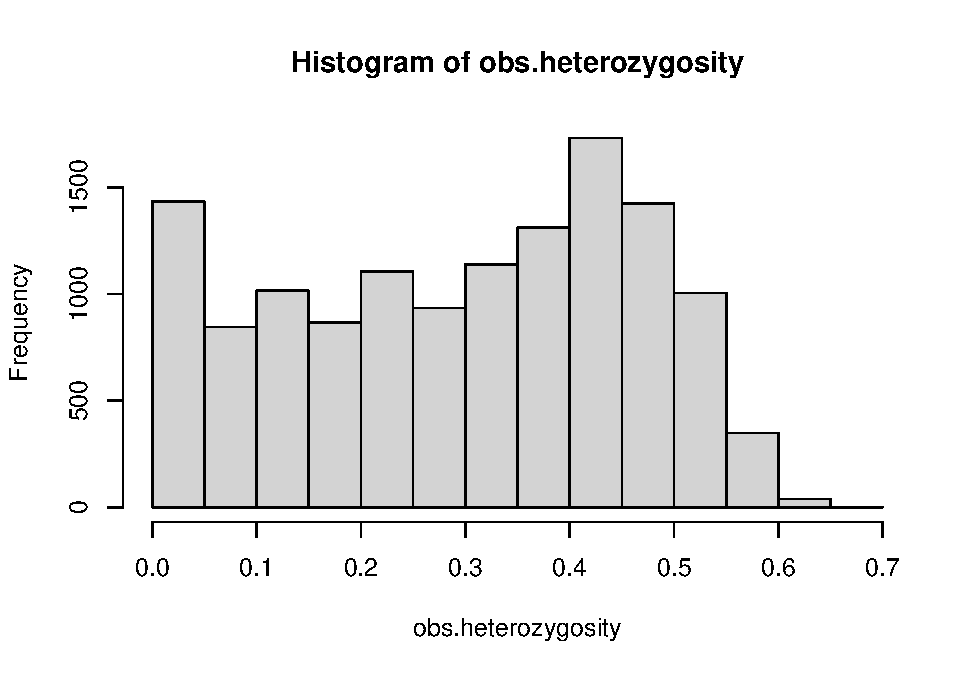
\includegraphics{P012020_Introduction_files/figure-latex/8th-1.pdf}

Theoretically the variation of this statistic can be in interval {[}0,
1.0{]} because H\_o = f\_AB, and f\_AB can have frequency of 0 and also
frequency of 1.0.

\begin{enumerate}
\def\labelenumi{\arabic{enumi}.}
\setcounter{enumi}{8}
\tightlist
\item
  (2p) Compute for each marker its expected heterozygosity (\(H_e\)),
  where the expected heterozygosity for a bi-allelic marker is defined
  as \(1 - \sum_{i=1}^k p_i^2\), where \(p_i\) is the frequency of the
  \(i\)th allele. Make a histogram of the expected heterozygosity. What
  is, theoretically, the range of variation of this statistic? What is
  the average of \(H_e\) for this database?
\end{enumerate}

\begin{Shaded}
\begin{Highlighting}[]
\NormalTok{h.expected <-}\StringTok{ }\ControlFlowTok{function}\NormalTok{(x) \{}
\NormalTok{  x[x }\OperatorTok{==}\StringTok{ }\DecValTok{0}\NormalTok{] =}\StringTok{ "AA"}
\NormalTok{  x[x }\OperatorTok{==}\StringTok{ }\DecValTok{1}\NormalTok{] =}\StringTok{ "AB"}
\NormalTok{  x[x }\OperatorTok{==}\StringTok{ }\DecValTok{2}\NormalTok{] =}\StringTok{ "BB"}
\NormalTok{  x <-}\StringTok{ }\KeywordTok{genotype}\NormalTok{(x,}\DataTypeTok{sep=}\StringTok{""}\NormalTok{)}
\NormalTok{  out <-}\StringTok{ }\KeywordTok{summary}\NormalTok{(x)}
  
\NormalTok{  res =}\StringTok{ }\FloatTok{1.0}
  \ControlFlowTok{for}\NormalTok{(p }\ControlFlowTok{in}\NormalTok{ out}\OperatorTok{$}\NormalTok{allele.freq[,}\DecValTok{2}\NormalTok{]) \{}
\NormalTok{    res =}\StringTok{ }\NormalTok{res }\OperatorTok{-}\StringTok{ }\NormalTok{p}\OperatorTok{*}\NormalTok{p}
\NormalTok{  \}}
  
  \KeywordTok{return}\NormalTok{(res)}
\NormalTok{\}}

\CommentTok{# Expected heterozygosity for all markers}
\NormalTok{hetero.expected =}\StringTok{ }\KeywordTok{apply}\NormalTok{(genetic_dataset_non_monomorphic, }\DecValTok{2}\NormalTok{, h.expected)}
\KeywordTok{hist}\NormalTok{(hetero.expected)}
\end{Highlighting}
\end{Shaded}

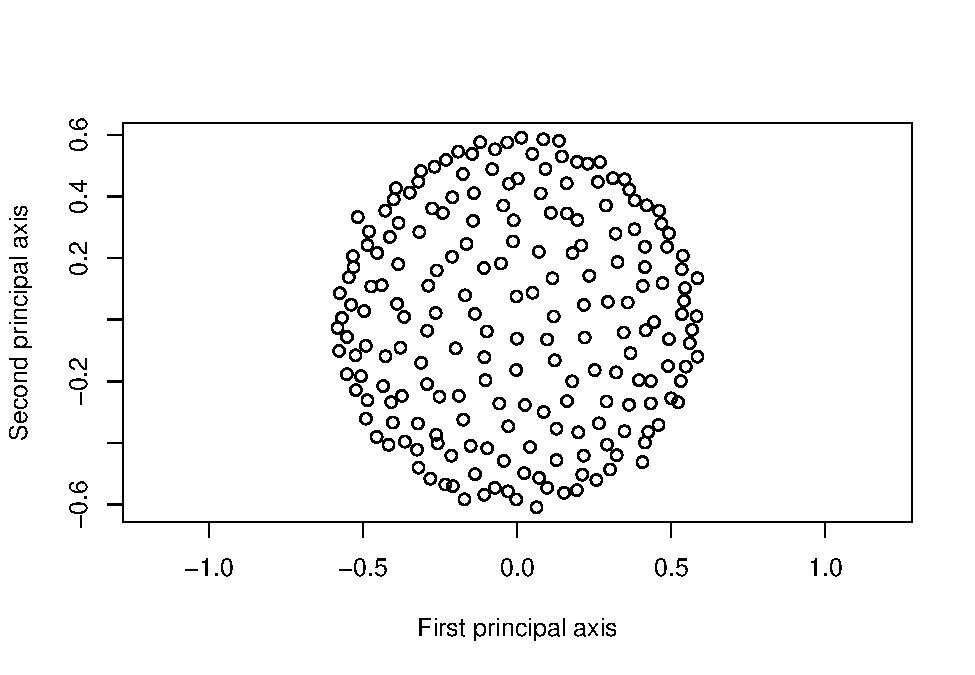
\includegraphics{P012020_Introduction_files/figure-latex/9th-1.pdf}

\begin{Shaded}
\begin{Highlighting}[]
\CommentTok{# Average heterozygosity}
\NormalTok{avg.hetero =}\StringTok{ }\KeywordTok{sum}\NormalTok{(hetero.expected) }\OperatorTok{/}\StringTok{ }\KeywordTok{length}\NormalTok{(hetero.expected)}
\KeywordTok{cat}\NormalTok{(}\KeywordTok{paste}\NormalTok{(}\StringTok{'The average H_e for this database is :'}\NormalTok{, avg.hetero))}
\end{Highlighting}
\end{Shaded}

\begin{verbatim}
## The average H_e for this database is : 0.298501117356988
\end{verbatim}

Theoretically the variation of this statistic depends on number of
alleles. In this case it can be in interval {[}0,0.5{]}. But in case of
4 alleles it can be anywhere between {[}0, 0.75{]}. The average expected
heterozygosity for this data-set is 0.2985.

\hypertarget{str-dataset-10p}{%
\section{STR dataset (10p)}\label{str-dataset-10p}}

\begin{enumerate}
\def\labelenumi{\arabic{enumi}.}
\tightlist
\item
  The file
  \href{http://www-eio.upc.es/~jan/data/bsg/FrenchStrs.dat}{FrenchStrs.dat}
  contains genotype information (STRs) of individuals from a French
  population. The first column of the data set contains an identifier
  the individual. STR data starts at the second column. Load this data
  into the R environment.
\end{enumerate}

\begin{Shaded}
\begin{Highlighting}[]
\NormalTok{French =}\StringTok{ }\KeywordTok{read.table}\NormalTok{(}\StringTok{"FrenchStrs.dat"}\NormalTok{)}
\NormalTok{dataset =}\StringTok{ }\NormalTok{French[,}\DecValTok{2}\OperatorTok{:}\KeywordTok{ncol}\NormalTok{(French)]}
\end{Highlighting}
\end{Shaded}

\begin{enumerate}
\def\labelenumi{\arabic{enumi}.}
\setcounter{enumi}{1}
\tightlist
\item
  (1p) How many individuals and how many STRs contains the database?
\end{enumerate}

\begin{Shaded}
\begin{Highlighting}[]
\NormalTok{n =}\StringTok{ }\KeywordTok{nrow}\NormalTok{(dataset) }\OperatorTok{/}\StringTok{ }\DecValTok{2} \CommentTok{# 2 rows for each individual}
\NormalTok{strs =}\StringTok{ }\KeywordTok{ncol}\NormalTok{(dataset)}
\KeywordTok{cat}\NormalTok{(}\KeywordTok{paste}\NormalTok{(}\StringTok{'Number of individuals: '}\NormalTok{, n, }\StringTok{'}\CharTok{\textbackslash{}n}\StringTok{'}\NormalTok{))}
\end{Highlighting}
\end{Shaded}

\begin{verbatim}
## Number of individuals:  29
\end{verbatim}

\begin{Shaded}
\begin{Highlighting}[]
\KeywordTok{cat}\NormalTok{(}\KeywordTok{paste}\NormalTok{(}\StringTok{'Number of STRs: '}\NormalTok{, strs))}
\end{Highlighting}
\end{Shaded}

\begin{verbatim}
## Number of STRs:  678
\end{verbatim}

\begin{enumerate}
\def\labelenumi{\arabic{enumi}.}
\setcounter{enumi}{2}
\tightlist
\item
  (1p) The value \(-9\) indicates a missing value. Replace all missing
  values by NA. What percentage of the total amount of datavalues is
  missing?
\end{enumerate}

\begin{Shaded}
\begin{Highlighting}[]
\NormalTok{dataset[dataset }\OperatorTok{==}\StringTok{ }\DecValTok{-9}\NormalTok{] =}\StringTok{ }\OtherTok{NA}

\NormalTok{n.mis =}\StringTok{ }\KeywordTok{sum}\NormalTok{(}\KeywordTok{is.na}\NormalTok{(dataset))}
\NormalTok{n.total =}\StringTok{ }\KeywordTok{nrow}\NormalTok{(dataset) }\OperatorTok{*}\StringTok{ }\NormalTok{(}\KeywordTok{ncol}\NormalTok{(dataset))}

\NormalTok{perc.mis =}\StringTok{ }\NormalTok{n.mis }\OperatorTok{/}\StringTok{ }\NormalTok{n.total}
\KeywordTok{cat}\NormalTok{(}\KeywordTok{paste}\NormalTok{(}\StringTok{'Percentage of missing values: '}\NormalTok{, }\KeywordTok{round}\NormalTok{(perc.mis}\OperatorTok{*}\DecValTok{100}\NormalTok{, }\DecValTok{2}\NormalTok{), }\StringTok{'%}\CharTok{\textbackslash{}n}\StringTok{'}\NormalTok{))}
\end{Highlighting}
\end{Shaded}

\begin{verbatim}
## Percentage of missing values:  4.21 %
\end{verbatim}

\begin{enumerate}
\def\labelenumi{\arabic{enumi}.}
\setcounter{enumi}{3}
\tightlist
\item
  (2p) Write a function that determines the number of alleles for a STR.
  Determine the number of alleles for each STR in the database. Compute
  basic descriptive statistics of the number of alleles (mean, standard
  deviation, median, minimum, maximum).
\end{enumerate}

\begin{Shaded}
\begin{Highlighting}[]
\NormalTok{n.alleles <-}\StringTok{ }\ControlFlowTok{function}\NormalTok{(x) \{}
  \KeywordTok{length}\NormalTok{(}\KeywordTok{unique}\NormalTok{(x[}\OperatorTok{!}\KeywordTok{is.na}\NormalTok{(x)]))}
\NormalTok{\}}

\NormalTok{n.alleles.per.STR =}\StringTok{ }\KeywordTok{apply}\NormalTok{(dataset, }\DecValTok{2}\NormalTok{, n.alleles)}

\KeywordTok{cat}\NormalTok{(}\KeywordTok{paste}\NormalTok{(}\StringTok{'Standard deviation: '}\NormalTok{, }\KeywordTok{sd}\NormalTok{(n.alleles.per.STR), }\StringTok{'}\CharTok{\textbackslash{}n}\StringTok{'}\NormalTok{))}
\end{Highlighting}
\end{Shaded}

\begin{verbatim}
## Standard deviation:  1.82338480266172
\end{verbatim}

\begin{Shaded}
\begin{Highlighting}[]
\KeywordTok{cat}\NormalTok{(}\StringTok{'Other descriptive statistics: }\CharTok{\textbackslash{}n}\StringTok{'}\NormalTok{)}
\end{Highlighting}
\end{Shaded}

\begin{verbatim}
## Other descriptive statistics:
\end{verbatim}

\begin{Shaded}
\begin{Highlighting}[]
\KeywordTok{summary}\NormalTok{(n.alleles.per.STR)}
\end{Highlighting}
\end{Shaded}

\begin{verbatim}
##    Min. 1st Qu.  Median    Mean 3rd Qu.    Max. 
##   3.000   5.000   6.000   6.375   7.000  16.000
\end{verbatim}

\begin{Shaded}
\begin{Highlighting}[]
\KeywordTok{boxplot}\NormalTok{(n.alleles.per.STR, }\DataTypeTok{main=}\StringTok{'Box plot of number of alleles per STR'}\NormalTok{, }\DataTypeTok{ylab=}\StringTok{'Number of alleles'}\NormalTok{)}
\end{Highlighting}
\end{Shaded}

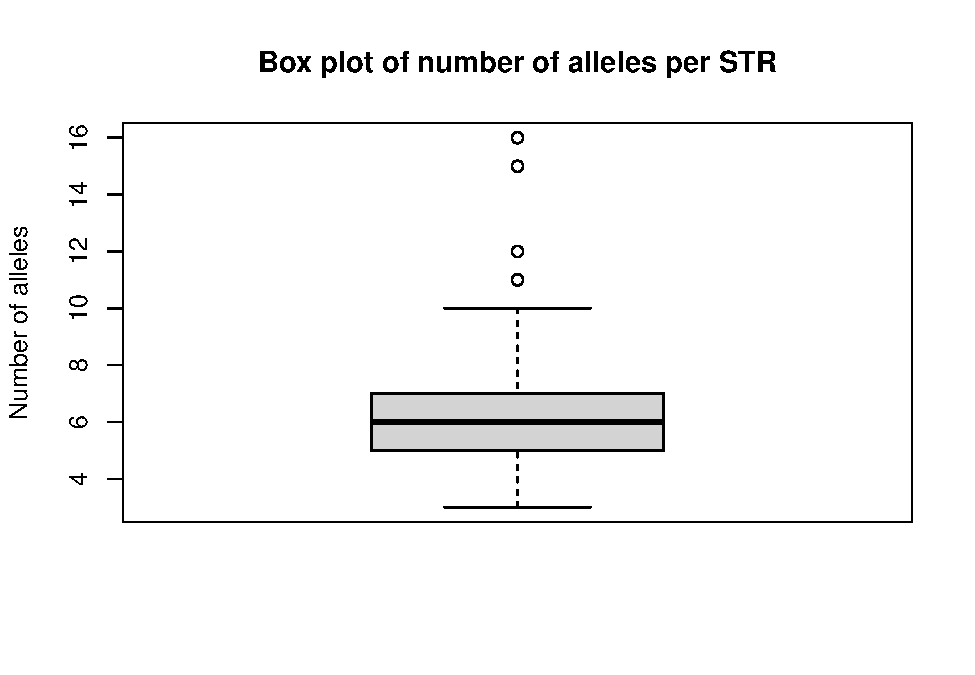
\includegraphics{P012020_Introduction_files/figure-latex/str4th-1.pdf}

\begin{enumerate}
\def\labelenumi{\arabic{enumi}.}
\setcounter{enumi}{4}
\tightlist
\item
  (2p) Make a table with the number of STRs for a given number of
  alleles and present a barplot of the number STRs in each category.
  What is the most common number of alleles for an STR?
\end{enumerate}

\begin{Shaded}
\begin{Highlighting}[]
\NormalTok{allele.counts =}\StringTok{ }\KeywordTok{sort}\NormalTok{(}\KeywordTok{unique}\NormalTok{(n.alleles.per.STR))}
\NormalTok{str.counts =}\StringTok{ }\KeywordTok{c}\NormalTok{()}

\ControlFlowTok{for}\NormalTok{(c }\ControlFlowTok{in}\NormalTok{ allele.counts) \{}
\NormalTok{  num =}\StringTok{ }\KeywordTok{sum}\NormalTok{(n.alleles.per.STR }\OperatorTok{==}\StringTok{ }\NormalTok{c)}
\NormalTok{  str.counts =}\StringTok{ }\KeywordTok{append}\NormalTok{(str.counts, num)}
\NormalTok{\}}

\KeywordTok{barplot}\NormalTok{(str.counts, }\DataTypeTok{names.arg=}\NormalTok{allele.counts, }\DataTypeTok{main=}\StringTok{'Number of STRs for specified number of alleles'}\NormalTok{, }\DataTypeTok{xlab=}\StringTok{'Number of alleles'}\NormalTok{, }\DataTypeTok{ylab=}\StringTok{'Frequency'}\NormalTok{)}
\end{Highlighting}
\end{Shaded}

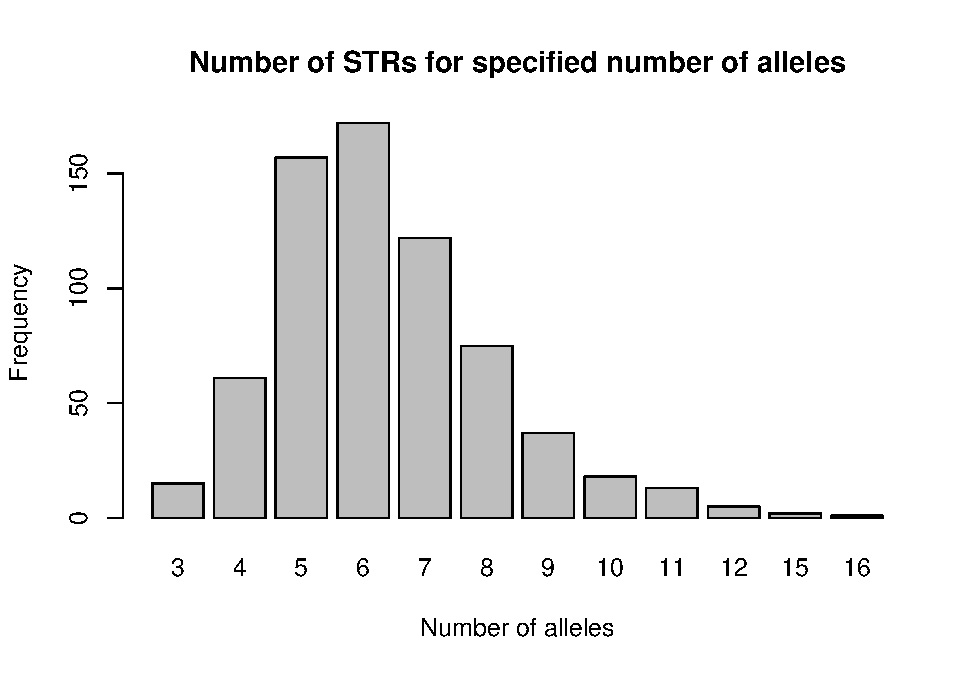
\includegraphics{P012020_Introduction_files/figure-latex/str5th-1.pdf}

Most common number of alleles for a STR is 6.

\begin{enumerate}
\def\labelenumi{\arabic{enumi}.}
\setcounter{enumi}{5}
\tightlist
\item
  (2p) Compute the expected heterozygosity for each STR. Make a
  histogram of the expected heterozygosity over all STRS. Compute the
  average expected heterozygosity over all STRs.
\end{enumerate}

\begin{Shaded}
\begin{Highlighting}[]
\NormalTok{h.expected.str <-}\StringTok{ }\ControlFlowTok{function}\NormalTok{(x) \{}
\NormalTok{  x =}\StringTok{ }\NormalTok{x[}\OperatorTok{!}\KeywordTok{is.na}\NormalTok{(x)]}
\NormalTok{  tbl =}\StringTok{ }\KeywordTok{table}\NormalTok{(x)}
\NormalTok{  total =}\StringTok{ }\KeywordTok{sum}\NormalTok{(tbl)}
\NormalTok{  result =}\StringTok{ }\FloatTok{1.0}
  \ControlFlowTok{for}\NormalTok{(t }\ControlFlowTok{in}\NormalTok{ tbl) \{}
\NormalTok{    result =}\StringTok{ }\NormalTok{result }\OperatorTok{-}\StringTok{ }\NormalTok{(t}\OperatorTok{/}\NormalTok{total)}\OperatorTok{^}\DecValTok{2}
\NormalTok{  \}}
\NormalTok{  result}
\NormalTok{\}}


\NormalTok{h.expected.per.STR =}\StringTok{ }\KeywordTok{apply}\NormalTok{(dataset, }\DecValTok{2}\NormalTok{, h.expected.str)}
\NormalTok{he.df <-}\StringTok{ }\KeywordTok{data.frame}\NormalTok{(h.expected.per.STR)}
\KeywordTok{names}\NormalTok{(he.df)=}\KeywordTok{c}\NormalTok{(}\StringTok{'Expected heterozygosity'}\NormalTok{)}
\CommentTok{#(he.df)}


\KeywordTok{hist}\NormalTok{(h.expected.per.STR, }\DataTypeTok{main=}\StringTok{'Histogram of Expected Heterozygosity per STR'}\NormalTok{, }\DataTypeTok{xlab=}\StringTok{'Expected heterozygosity per STR'}\NormalTok{)}
\end{Highlighting}
\end{Shaded}

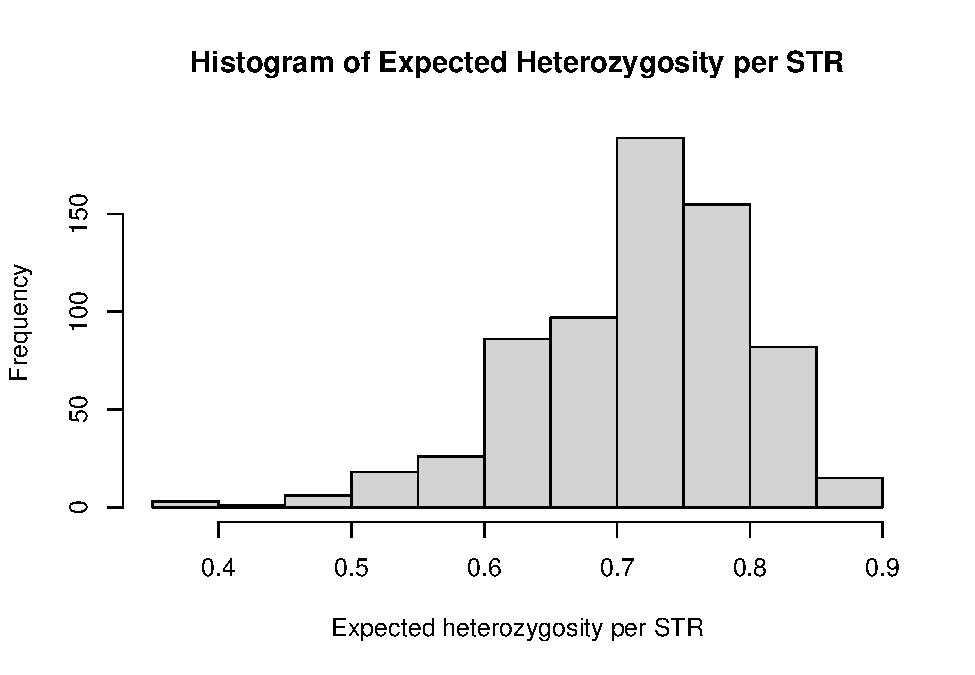
\includegraphics{P012020_Introduction_files/figure-latex/str6th-1.pdf}

\begin{Shaded}
\begin{Highlighting}[]
\KeywordTok{cat}\NormalTok{(}\KeywordTok{paste}\NormalTok{(}\StringTok{'Average expected heterozygosity over all STR: '}\NormalTok{, }\KeywordTok{mean}\NormalTok{(h.expected.per.STR)))}
\end{Highlighting}
\end{Shaded}

\begin{verbatim}
## Average expected heterozygosity over all STR:  0.717266239372483
\end{verbatim}

\begin{enumerate}
\def\labelenumi{\arabic{enumi}.}
\setcounter{enumi}{6}
\tightlist
\item
  (2p) Compare the results you obtained for the SNP database with those
  you obtained for the STR database. What differences do you observe
  between these two types of genetic markers?
\end{enumerate}

When comparing SNP and STR databases, we can observe that SNP database
has much more variants (16393) then STR database (678). While the SNP
database does not have any missing values, there is 4.2\% of data
missing in the STR database.

Variants of SNP contain only 2 different alleles and therefore 3
different genotypes, while average number of alleles in STR variants is
around 6. Higher number of alleles is the reason why STR's expected
heterozygosity can theoretically be and is higher than SNP's.

\end{document}
